\let\negmedspace\undefined
\let\negthickspace\undefined
\documentclass[journal]{IEEEtran}
\usepackage[a5paper, margin=10mm, onecolumn]{geometry}
%\usepackage{lmodern} % Ensure lmodern is loaded for pdflatex
\usepackage{tfrupee} % Include tfrupee package
\setlength{\headheight}{1cm} % Set the height of the header box
\setlength{\headsep}{0mm}     % Set the distance between the header box and the top of the text
\usepackage{gvv-book}
\usepackage{gvv}
\usepackage{cite}
\usepackage{amsmath,amssymb,amsfonts,amsthm}
\usepackage{algorithmic}
\usepackage{graphicx}
\usepackage{textcomp}
\usepackage{xcolor}
\usepackage{txfonts}
\usepackage{listings}
\usepackage{enumitem}
\usepackage{mathtools}
\usepackage{gensymb}
\usepackage{comment}
\usepackage[breaklinks=true]{hyperref}
\usepackage{tkz-euclide} 
\usepackage{listings}
% \usepackage{gvv}                                        
\def\inputGnumericTable{}                                 
\usepackage[latin1]{inputenc}                                
\usepackage{color}                                            
\usepackage{array}                                            
\usepackage{longtable}                                       
\usepackage{calc}                                             
\usepackage{multirow}                                         
\usepackage{hhline}                                           
\usepackage{ifthen}                                           
\usepackage{lscape}
\usepackage{circuitikz}
\tikzstyle{block} = [rectangle, draw, fill=blue!20, 
    text width=4em, text centered, rounded corners, minimum height=3em]
\tikzstyle{sum} = [draw, fill=blue!10, circle, minimum size=1cm, node distance=1.5cm]
\tikzstyle{input} = [coordinate]
\tikzstyle{output} = [coordinate]
\begin{document}
\bibliographystyle{IEEEtran}
\vspace{3cm}
\title{10.7.26}
\author{AI25BTECH11017-BALU}
 \maketitle
% \newpage
% \bigskip
{\let\newpage\relax\maketitle}
\renewcommand{\thefigure}{\theenumi}
\renewcommand{\thetable}{\theenumi}
\setlength{\intextsep}{10pt} % Space between text and floats
\numberwithin{equation}{enumi}
\numberwithin{figure}{enumi}
\renewcommand{\thetable}{\theenumi}
\textbf{Question}:\\
\begin{enumerate}
    \item The focal chord to \( y^2 = 16x \) is tangent to \( (x - 6)^2 + y^2 = 2 \), then the possible values of the slope of this chord are: (2003)
    \begin{enumerate}
        \item \( -1, 1 \)
        \item \( -2, 2 \)
        \item \( -2, -\frac{1}{2} \)
        \item \( 2, -\frac{1}{2} \)
    \end{enumerate}
\end{enumerate}
\solution \\
Let us solve the given equation theoretically and then verify the solution computationally \\
According to the question, \\
The parabola is
\begin{align}
y^{2} = 16x.
\end{align}
In quadratic form, this can be written as
\begin{align}
\vec{x}^{T}
\myvec{0 & 0 \\ 0 & 1}
\vec{x}
+
2\myvec{-8 \\ 0}^{T}\vec{x} = 0.
\end{align}
\begin{align}
\vec{x}^{T}\vec{I}\vec{x} + 2
\myvec{-6 \\ 0}^{T}\vec{x} + 34 = 0.
\end{align}
Thus,
\begin{align}
\vec{V} = \vec{I},\quad
\vec{u} = \myvec{-6 \\ 0},\quad
f = 34.
\end{align}

The focus of the parabola is
\begin{align}
\vec{F} = \myvec{4 \\ 0}.
\end{align}
tangency condition
\begin{align}
    \vec{m}^T(\vec{q}\vec{v}+\vec{u})=0\\
    \vec{q} \text{is point of contact}\\
    \end{align}
     \text{equation of tangent}\\
    \begin{align}
    (\vec{q}\vec{v}+\vec{u})^T\vec{x}+\vec{u}^T\vec{q}+f=0
\end{align}
\begin{align}
    \vec{m}^T(\vec{q}\vec{v}+\vec{u})=0\\ 
    (\vec{q}\vec{v}+\vec{u})^T\vec{F}+\vec{u}^T\vec{q}+f=0\\
    \vec{q}^{T}\vec{v}\vec{q} + 2
\myvec{-6 \\ 0}^{T}\vec{q} + 34 = 0.
\end{align}
by solving above equations we get\\
$m=1,-1$





\begin{figure}[h!]
    \centering
    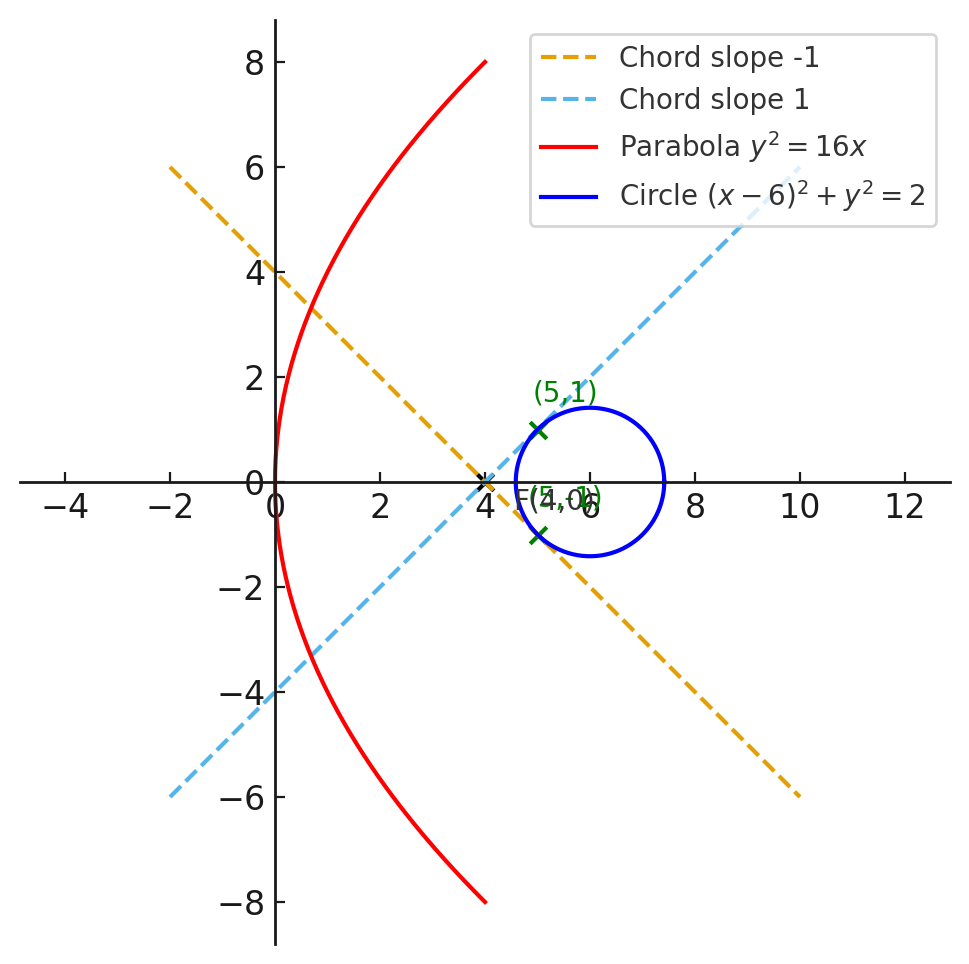
\includegraphics[width=0.5\linewidth]{figs/tangent.png}
    \caption{}
    \label{fig:placeholder}
\end{figure}
\end{document}